\documentclass[14pt, table]{extarticle}
\usepackage{amsfonts}
\usepackage{amsmath}
\usepackage[utf8]{inputenc}
\usepackage[a4paper, total={7in, 10.5in}]{geometry}
\usepackage[table]{xcolor}
\usepackage{tgbonum}
\usepackage{float}
\usepackage{graphicx}
\graphicspath{ {./images/} }
\DeclareGraphicsExtensions{.png,.jpg}
\usepackage{caption}
\usepackage{tikz}
\usepackage{circuitikz}
\usepackage[T1]{fontenc}
\usetikzlibrary{quotes,angles}
\usetikzlibrary{arrows}

\title{\textbf{Sprawozdanie} \\ \Large{Ćwiczenie 1}}
\date{Data wykonania: 15 marca 2023}
\author{ \Large{Jan Kwinta} \\ \large{Prowadzący ćwiczenia: prof. Jerzy Smyrski}}


\newcommand{\nl}{\vspace{0.5cm}}
\newcommand{\nz}{\vspace{1.5cm}}
\newcommand{\zatem}{\textrm{Zatem }}

\definecolor{trueGreen}{HTML}{009900}

\begin{document}
\maketitle

\paragraph{Wstęp teoretyczny \\}
Podczas pierwszych labolatoriów z elektroniki cyfrowej zapoznawaliśmy się z narzędziami dostępnymi w pracowni elektronicznej: oscyloskopem Tektronix MSO3000 oraz generatorem przebiegów elektrycznych Tektronix AFG3000. W celu nauki podstaw obsługi tych urządzeń wykonaliśmy trzy zadania dotyczące:

\begin{itemize}
    \item Obserwacji i pomiaru kształtu funkcji, amplitudy, częstotliwości i przesunięcia fazowego sygnałów.
    \item Generowania i obserwacji dwóch funkcji harmonicznych tworzących krzywe Lissajous.
    \item Obserwacji zjawiska dudnienia, które powstaje przy sumowaniu dwóch sygnałów o zbliżonych częstotliwościach; pomiaru okresów wygenerowanych dudnień.
\end{itemize}

\newpage
\paragraph{Ćwiczenie 1.1 \\}
\textit{Obserwacja syngałów z generatora.} Pierwszym zadaniem było podanie sygnału z generatora na oscyloskop, obserwacja kształtu sygnału i zapisanie obrazu wyświetlanego na ekranie oscyloskopu. Poniżej zapisałem 3 obrazy: 

\begin{enumerate}
    \item Sygnał sinusoidalny o częstotliwości $3$ $kHz$ i amplitudzie $2$ $V$pp.
    \item Sygnał trójkątny o częstotliwości $3$ $kHz$ i amplitudzie $3$ $V$pp.
    \item Sygnał prostokątny o częstotliwości $2$ $kHz$ i amplitudzie $2$ $V$pp.
\end{enumerate}

\begin{figure}[H]
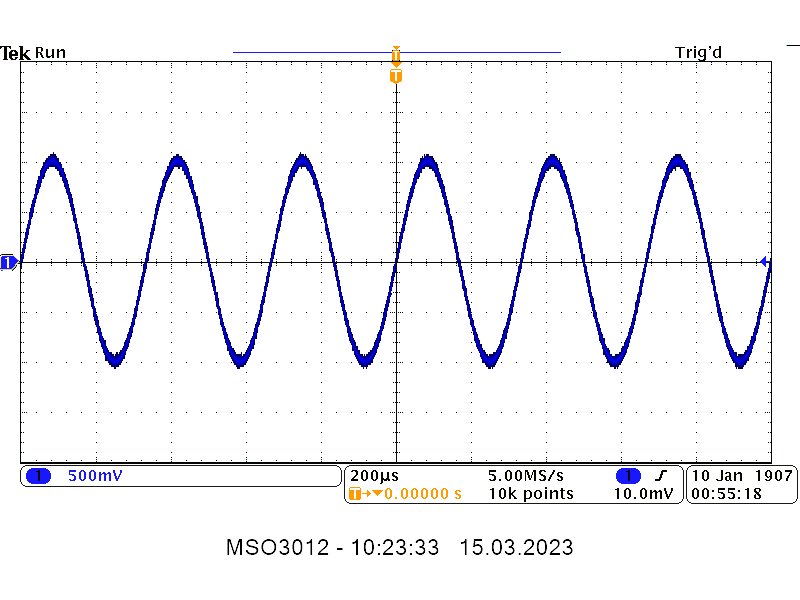
\includegraphics[scale=0.7]{A18}
\centering
\captionsetup{labelformat=empty}
\caption{1: Sygnał sinusoidalny.}
\end{figure}

\begin{figure}[H]
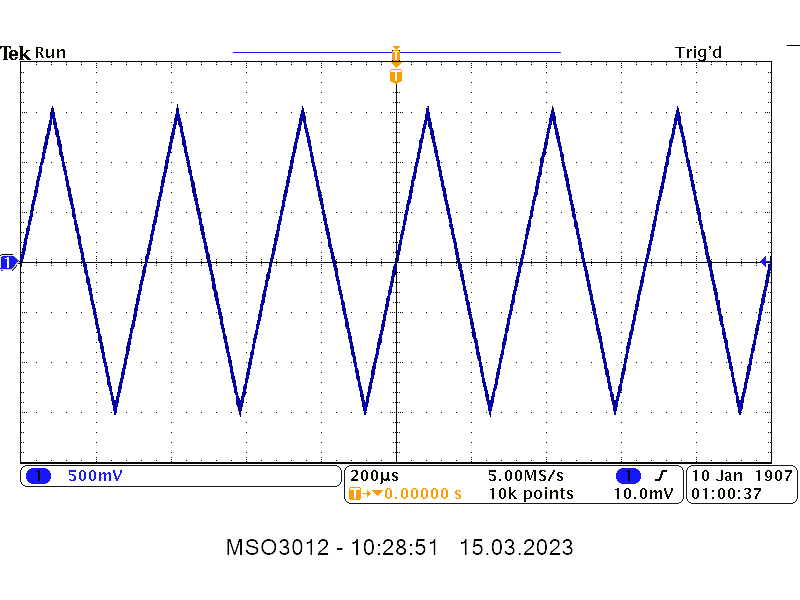
\includegraphics[scale=0.7]{A20}
\centering
\captionsetup{labelformat=empty}
\caption{2: Sygnał trójkątny.}
\end{figure}

\begin{figure}[H]
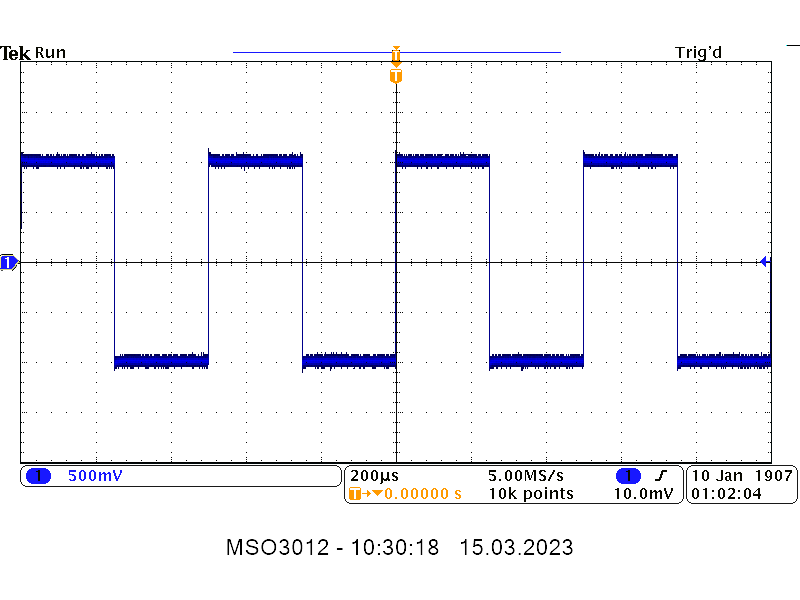
\includegraphics[scale=0.7]{A17}
\centering
\captionsetup{labelformat=empty}
\caption{3: Sygnał prostokątny.}
\end{figure}

\newpage
\textit{Pomiar amplitudy i częstotliwości sygnałów.} Oscyloskopem można wykonywać pomiary na kilka sposobów:

\begin{enumerate}
    \item W oparciu o poziome i pionowe działki wyświetlane na ekranie oscyloskopu. Działki poziome odpowiadają ustawionej wartości wzmocnienia sygnału, a działki pionowe podstawy czasu. Obydwie te wartości są widoczne u dołu ekranu.
    \item Za pomocą kursorów. Kursory to wbudowane w oscyloskop narzędzie służące do precyzyjnego mierzenia wartości takich jak: napięcie w danej chwili czasu, odstęp pomiędzy dwoma kursorami, itp.
    \item Za pomocą funkcji "Measure", która automatycznie analizuje sygnał i wyświetla na ekranie informacje o nim.
\end{enumerate}


\begin{figure}[H]
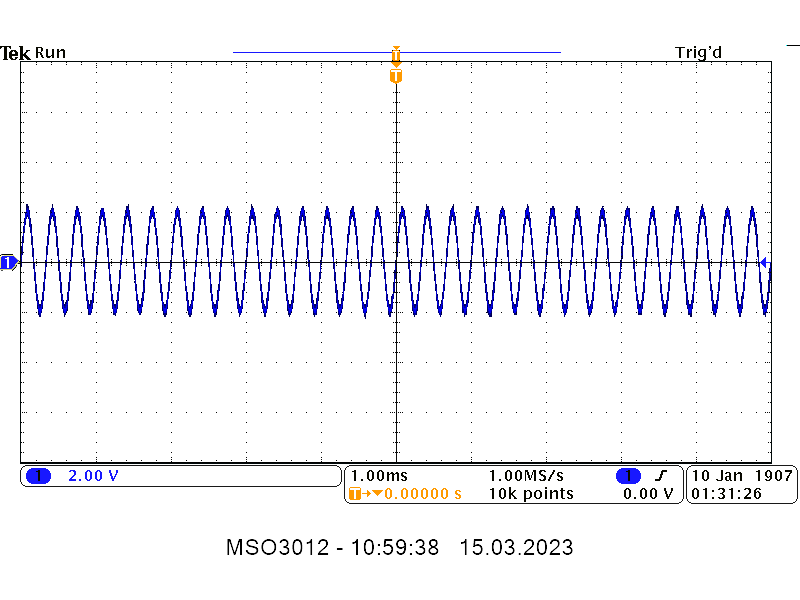
\includegraphics[scale=0.65]{A11}
\centering
\captionsetup{labelformat=empty}
\caption{Działki oscyloskopu: jednej działce na osi X odpowiada $1$ $ms$. W jednej działce czasu obserwujemy trzy przebiegi sygnału. Jednej działce na osi Y odpowiadają $2$ $V$. Możemy więc wnioskować, że sygnał ma częstotliwość $3$ $kHz$ i amplitudę $4$ $V$pp.}
\end{figure}

\newpage
\begin{figure}[H]
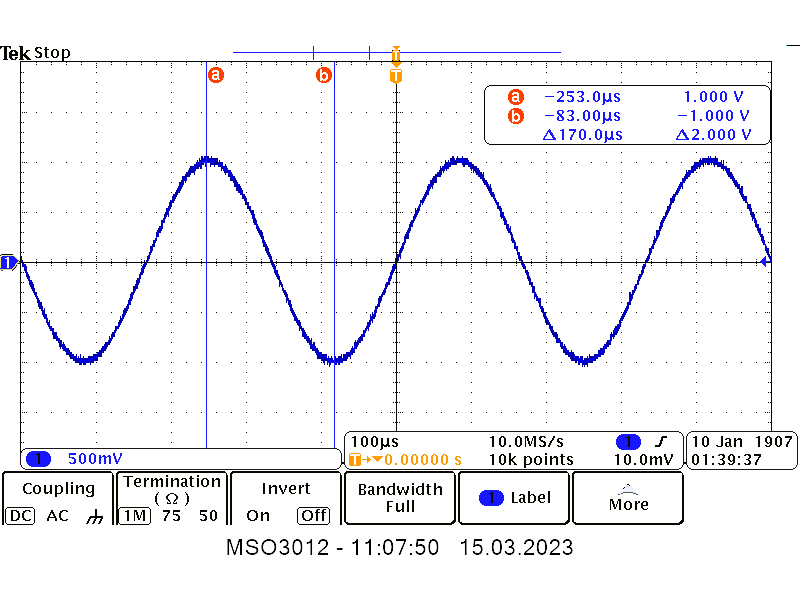
\includegraphics[scale=0.65]{A12}
\centering
\captionsetup{labelformat=empty}
\caption{Kursory: kursor A zmierzył wartość szczytową amplitudy $1$ $V$, zaś kursor B, wartość minimalną $-1$ $V$. Zatem amplituda \textit{peak-to-peak} tego sygnału wynosi $2$ $V$.}
\end{figure}

\begin{figure}[H]
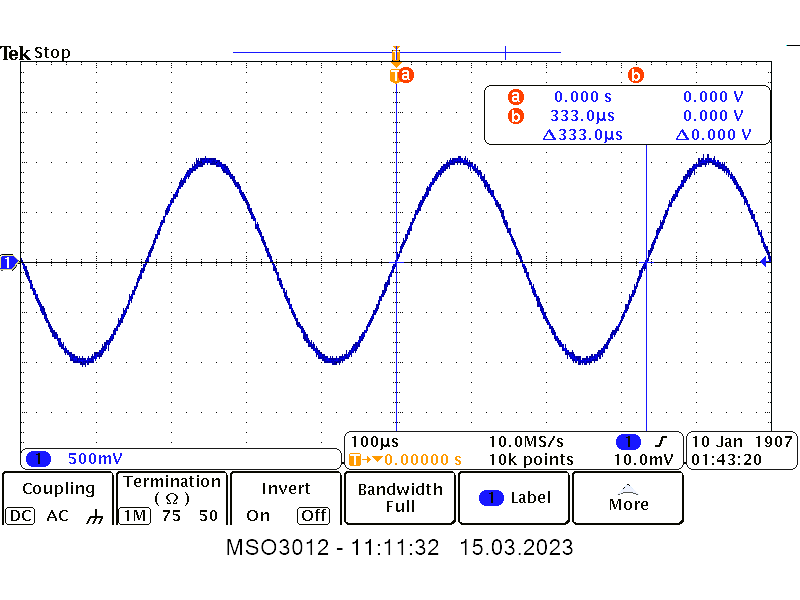
\includegraphics[scale=0.7]{A13}
\centering
\captionsetup{labelformat=empty}
\caption{Kursory: Siła sygnału w miejscu obydwu kursorów wynosi $0$ $V$. Odległość czasowa między kursorami to $333$ $\mu s$. Częstotliwość sygnału jest odwrotnością jego okresu, wynosi więc $\frac{1}{333 \cdot 10^{-6}} = \frac{1}{333} \cdot 10^6 \approx 3$ $kHz$.}
\end{figure}

\begin{figure}[H]
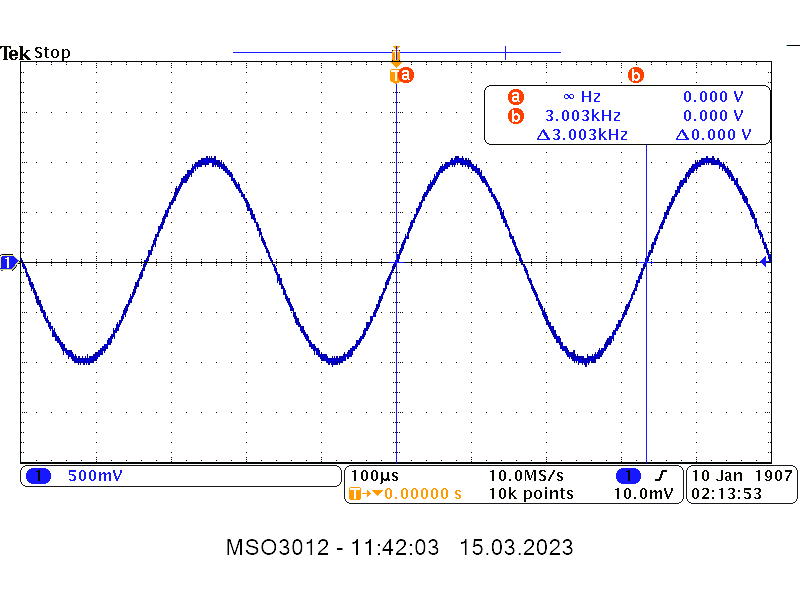
\includegraphics[scale=0.65]{A14}
\centering
\captionsetup{labelformat=empty}
\caption{Kursory: Powyższą metodę można też zastosować używając innej funkcji kursorów. Tu zamiast okresu sygnału oscyloskop od razu podaje częstotliwość.}
\end{figure}

\begin{figure}[H]
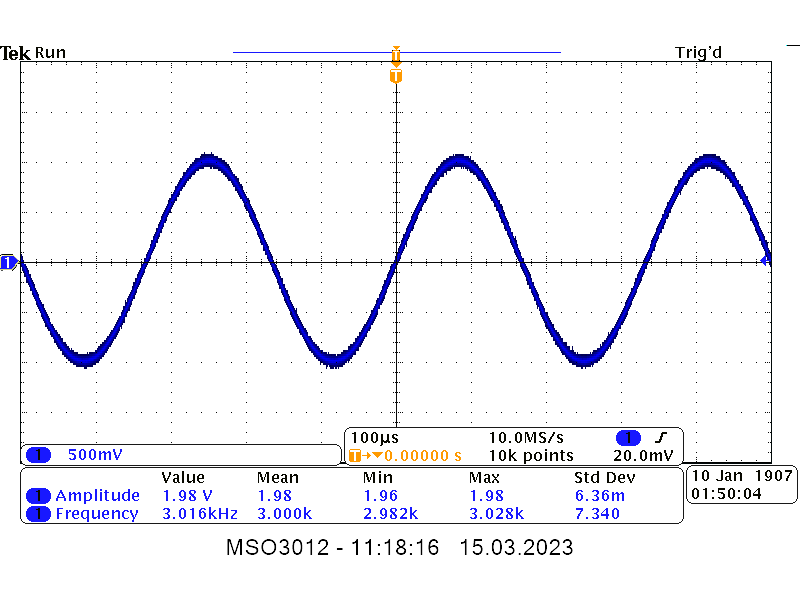
\includegraphics[scale=0.65]{A15}
\centering
\captionsetup{labelformat=empty}
\caption{Funkcja "Measure": Oscyloskop automatycznie podaje amplitudę ($1.98$ $V$) oraz częstotliwość ($3.016$ $kHz$) sygnału. Wyniki automatycznego pomiaru dosyć dokładnie odpowiadają wartościom ustawionym na generatorze: $2$ $V$ oraz $3$ $kHz$.}
\end{figure}

\newpage
\textit{Pomiar przesunięcia fazy.} Na kanały 1 i 2 oscyloskopu podane zostały dwa sygnały z wyjść 1 i 2 generatora. Obydwa sygnały sinusoidalne miały taką samą częstotliwość $3$ $kHz$ i taką samą amplitudę $2$ $V$pp. Wartość fazy sygnału została ustawiona na $0^{\circ}$ dla kanału 1 i $45^{\circ}$ dla kanału 2. \\

Tak ustawione przesunięcie fazowe można zmierzyć na dwa sposoby:
\begin{enumerate}
    \item Kursorami: ustawiając w menu kursorów jeden okres sygnału na kanale 1 jako $360^{\circ}$ i mierząc drugim kursorem przesunięcie przecięcia sygnału na kanale 2 z osią poziomą. Niestety nie zapisałem grafiki wykonania tego pomiaru.
    \item Za pomocą wbudowanej funkcji "Measure": ustawiając który sygnał chcemy mierzyć w stosunku do drugiego kanału.
\end{enumerate}

\begin{figure}[H]
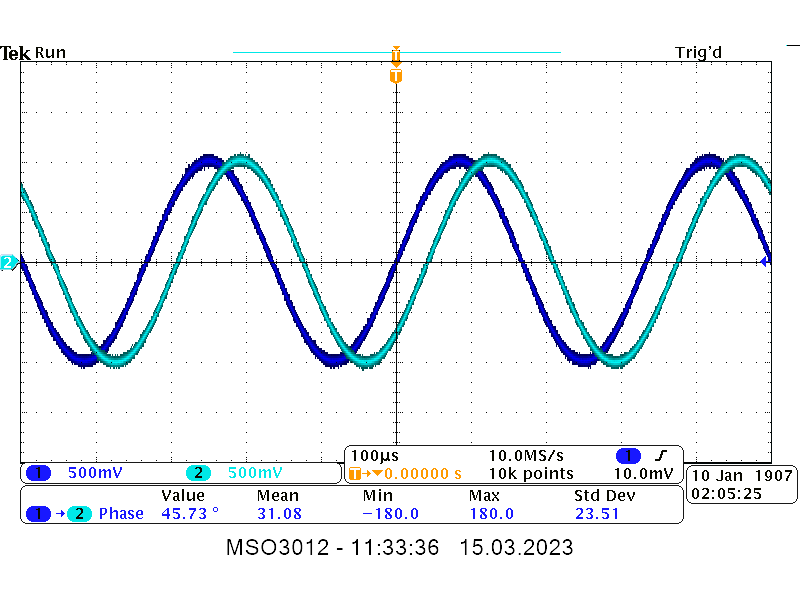
\includegraphics[scale=0.7]{A4}
\centering
\captionsetup{labelformat=empty}
\caption{Pomiar przesunięcia fazy dwóch sygnałów funkcją "Measure".}
\end{figure}

\newpage
\paragraph{Ćwiczenie 1.2 \\}
\textit{Krzywe Lissajous.} Wykorzystując tryb X-Y oscyloskopu możemy zaobserwować efekt złożenia dwóch drgań harmonicznych, które tworzą krzywe parametryzowane, zwane krzywymi Lissajous. Kształt krzywych zależy od stosunku częstotliwości dwóch sygnałów i ich przesunięcia fazy. W poniższych przykładach wybierałem na generatorze tę samą amplitudę dla obydwu kanałów ($2$ $V$) i różne częstotliwości oraz przesunięcia fazy. Kształty krzywych Lissajous mogą być bardzo różne, od mało skomplikowanych takich jak odcinek albo okrąg aż do złożonych zamkniętych krzywych przecinających się wiele razy.

\begin{figure}[H]
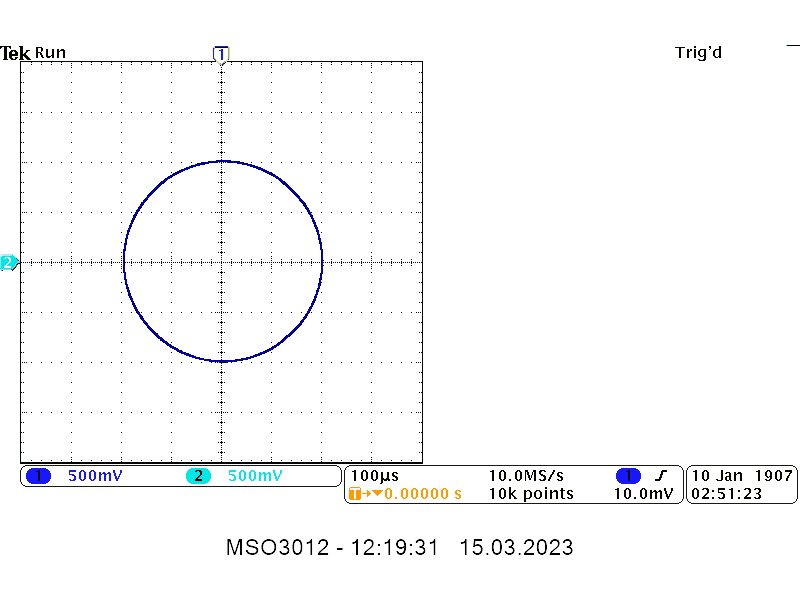
\includegraphics[scale=0.55]{A9}
\centering
\captionsetup{labelformat=empty}
\caption{Krzywa 1: kanał 1: $ 1$ $kHz$, kanał 2: $1 $ $kHz$, faza: $90^{\circ}$}
\end{figure}

\begin{figure}[H]
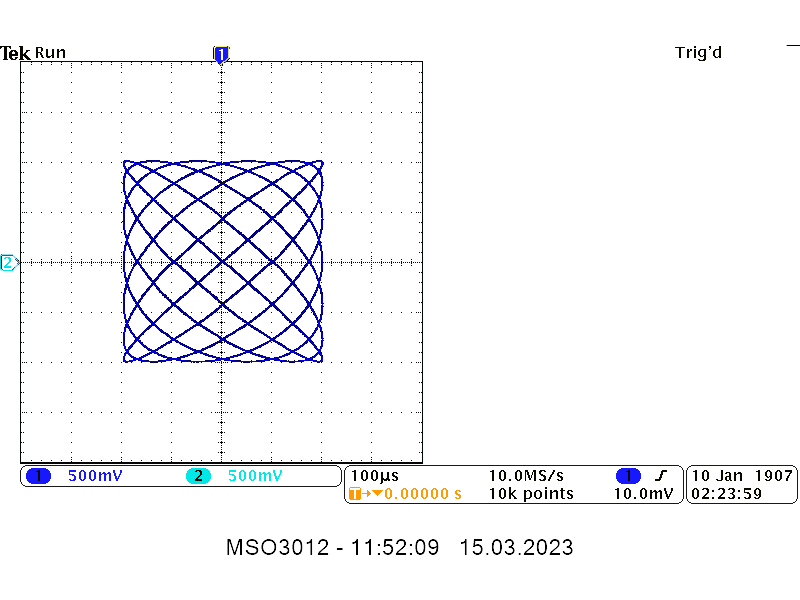
\includegraphics[scale=0.55]{A5}
\centering
\captionsetup{labelformat=empty}
\caption{Krzywa 2: kanał 1: $ 5$ $kHz$, kanał 2: $ 6$ $kHz$, faza: $0^{\circ}$}
\end{figure}

\begin{figure}[H]
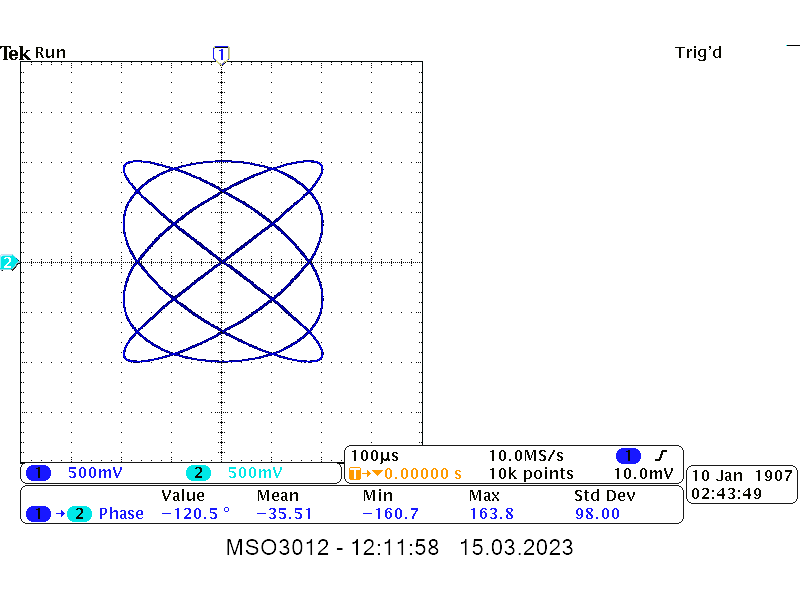
\includegraphics[scale=0.55]{A6}
\centering
\captionsetup{labelformat=empty}
\caption{Krzywa 3: kanał 1: $ 4$ $kHz$, kanał 2: $ 3$ $kHz$, faza: $180^{\circ}$}
\end{figure}

\begin{figure}[H]
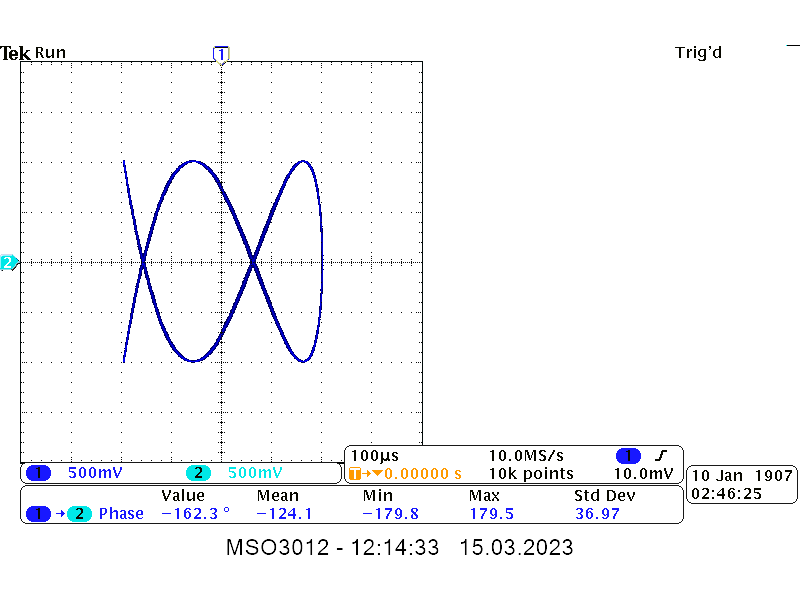
\includegraphics[scale=0.55]{A7}
\centering
\captionsetup{labelformat=empty}
\caption{Krzywa 4: kanał 1: $ 2$ $kHz$, kanał 2: $ 5$ $kHz$, faza: $90^{\circ}$}
\end{figure}

\begin{figure}[H]
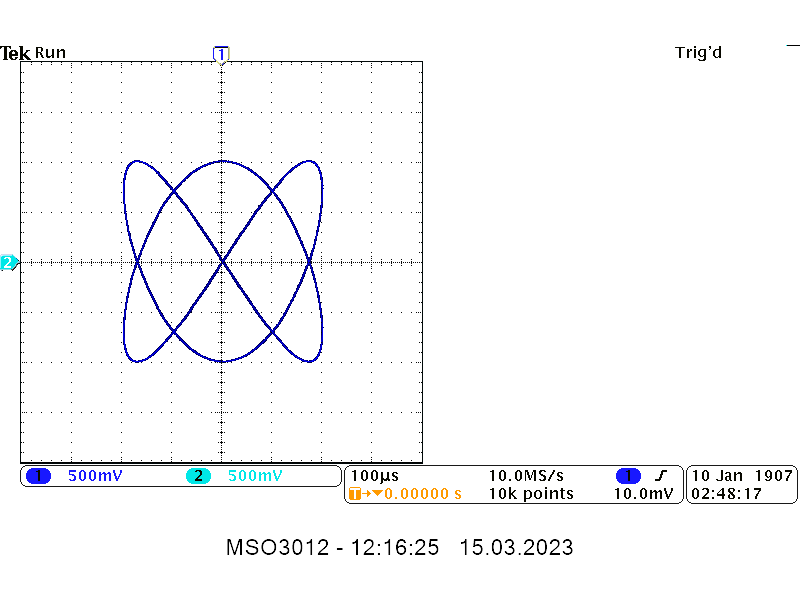
\includegraphics[scale=0.55]{A8}
\centering
\captionsetup{labelformat=empty}
\caption{Krzywa 5: kanał 1: $ $ 2$kHz$, kanał 2: $ 3$ $kHz$, faza: $120^{\circ}$}
\end{figure}

\begin{figure}[H]
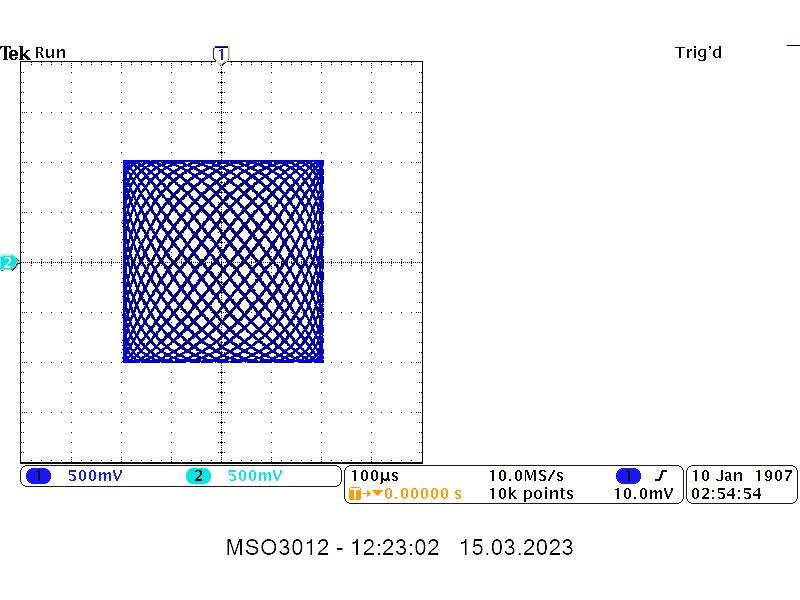
\includegraphics[scale=0.55]{A10}
\centering
\captionsetup{labelformat=empty}
\caption{Krzywa 6: kanał 1: $ 17$ $kHz$, kanał 2: $ 21$ $kHz$, faza: $6^{\circ}$}
\end{figure}

\newpage
\paragraph{Ćwiczenie 1.3 \\}
\textit{Dudnienia.} Jeżeli wykonamy sumowanie dwóch sygnałów sinusoidalnych o jednakowych amplitudach i zbliżonych (ale różnych) częstotliwościach możemy zaobserwować zjawisko dudnień.

\begin{figure}[H]
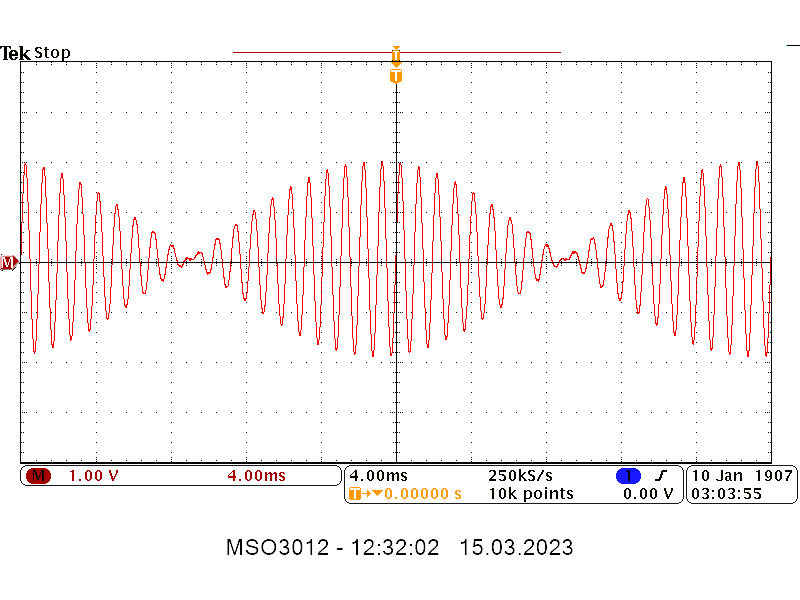
\includegraphics[scale=0.65]{A0}
\centering
\captionsetup{labelformat=empty}
\caption{Na kanale 1 sygnał o częstotliwości $1$ $kHZ$, na kanale 2 $1.05$ $kHz$. Obydwa sygnały mają amplitudę $2$ $V$pp.}
\end{figure}


Badając to zjawisko mierzymy dwie wartości: częstotliwość wypadkową $v_w$ oraz częstotliwość dudnień $v_d$. Okres wypadkowy $T_w = \frac{1}{v_w}$  to okres pomiędzy szczytami dwóch bliskich skoków. Okres dudnień $T_d = \frac{1}{v_d}$ wyznaczamy pomiędzy maksymalnymi skokami dudnień.\\ 

Jeżeli $v_1$ i $v_2$ to znane częstotliwości dodawanych sygnałów to możemy wyznaczyć częstotliwości analitycznie:

$$ v_w = \frac{v_1 + v_2}{2} $$ 
$$ v_d = \left| v_1 - v_2 \right| $$

W przypadku mierzonych przeze mnie dudnień sygnałów jest to:

$$ v_w = \frac{1 + 1.05}{2} = \frac{2.05}{2} = 1.025 \ [kHz]$$ 
$$ v_d = \left| 1 - 1.05 \right| = 0.05 \ [kHz] = 50 \ [Hz]$$

\newpage
Pomiary.

\begin{figure}[H]
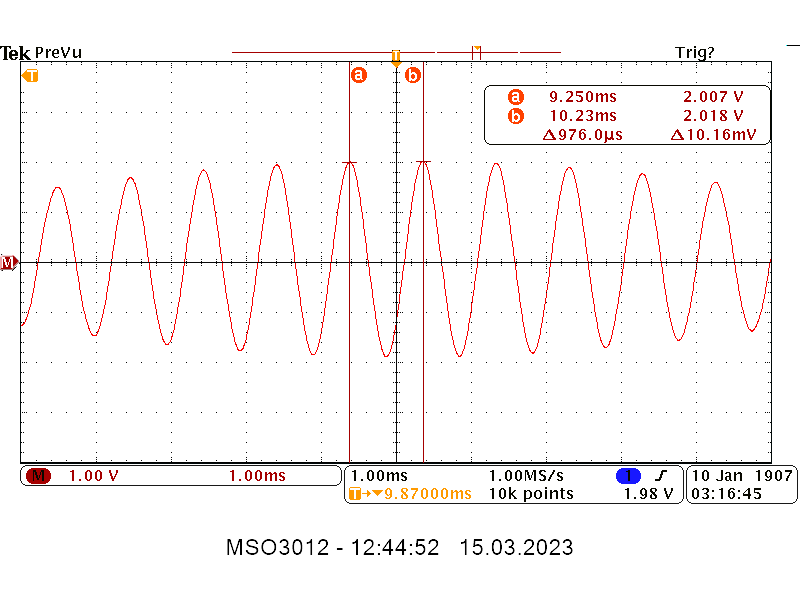
\includegraphics[scale=0.65]{A3}
\centering
\captionsetup{labelformat=empty}
\caption{Okres wypadkowy $T_w = 976 \ [\mu s]$.}
\end{figure}

Zatem $v_w = \frac{1}{976 \cdot 10^{-6}} \ [Hz] \approx 1024.59016 \ [Hz] = 1.024590 \ [kHz]$.

\begin{figure}[H]
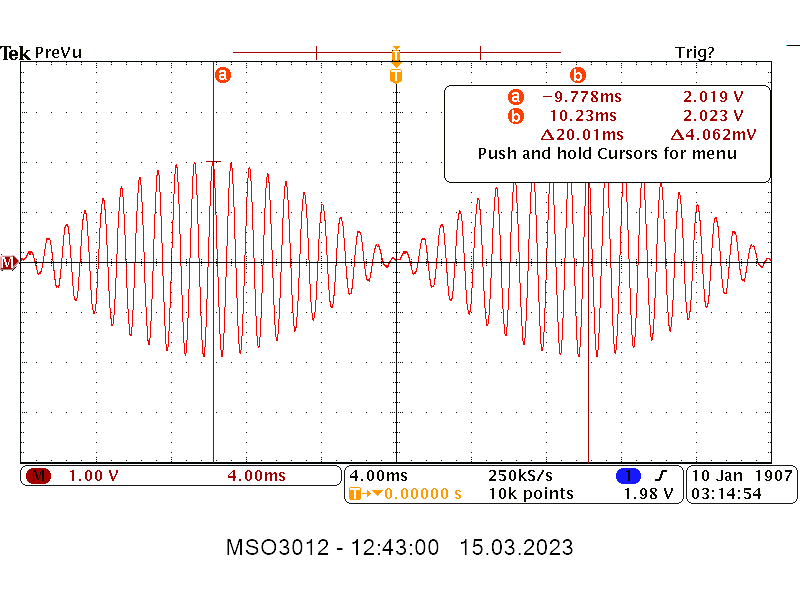
\includegraphics[scale=0.65]{A2}
\centering
\captionsetup{labelformat=empty}
\caption{Okres dudnień $T_d = 20.01 \ [ms]$.}
\end{figure}

Zatem $v_d = \frac{1}{20.01 \cdot 10^{-3}} \ [Hz] \approx 49.975012 \ [Hz] $.

\newpage
\paragraph{Omówienie wyników \\}

Podczas pomiarów amplitudy i częstotliwości sygnałów (Ćwiczenie 1.1) za pomocą kursorów oscyloskop wskazywał wartości z błędem względnym rzędu $0.1\%$ w porównaniu do parametrów ustawionych na generatorze przebiegów.

$$ \textrm{Dla częstotliwości: } \left| \frac{3000 - 3003}{3000} \right| = 0.1\% $$

Funkcja "Measure" oscyloskopu przy mierzeniu amplitudy, częstotliwości i przesunięcia fazy wykazała nieco większy błąd.

$$ \textrm{Dla częstotliwości: } \left| \frac{3000 - 3016}{3000} \right| = 0.53\% $$
$$ \textrm{Dla amplitudy: } \left| \frac{2 - 1.98}{2} \right| = 0.1\% $$
$$ \textrm{Dla przesunięcia fazy: } \left| \frac{45 - 45.73}{45} \right| = 0.162\% $$

Warto również zaznaczyć, że oscyloskop posiada więcej narzędzi, do mierzenia nawet najmniejszych zmian sygnału, np automatyczne obliczanie średniej i odchylenia standardowego mierzonej wartości w danym zakresie czasu. \\

Przy obliczaniu częstotliwości dudnień błąd wyników moich pomiarów w stosunku do obliczonych analitycznie "idealnych" częstotliwości był mniejszy niż $0.05\%$.

$$ \left| \frac{1.025 - 1.02459}{1.025} \right| = 0.04\% $$
$$ \left| \frac{50 - 49.975012}{50} \right| = 0.049976\% $$


\newpage
\paragraph{Notatki z zeszytu labolatoryjnego \\}
Poniżej załączone są notatki z zeszytu labolatoryjnego, które prowadziłem podczas zajęć wykonując pomiary.

\begin{figure}[H]
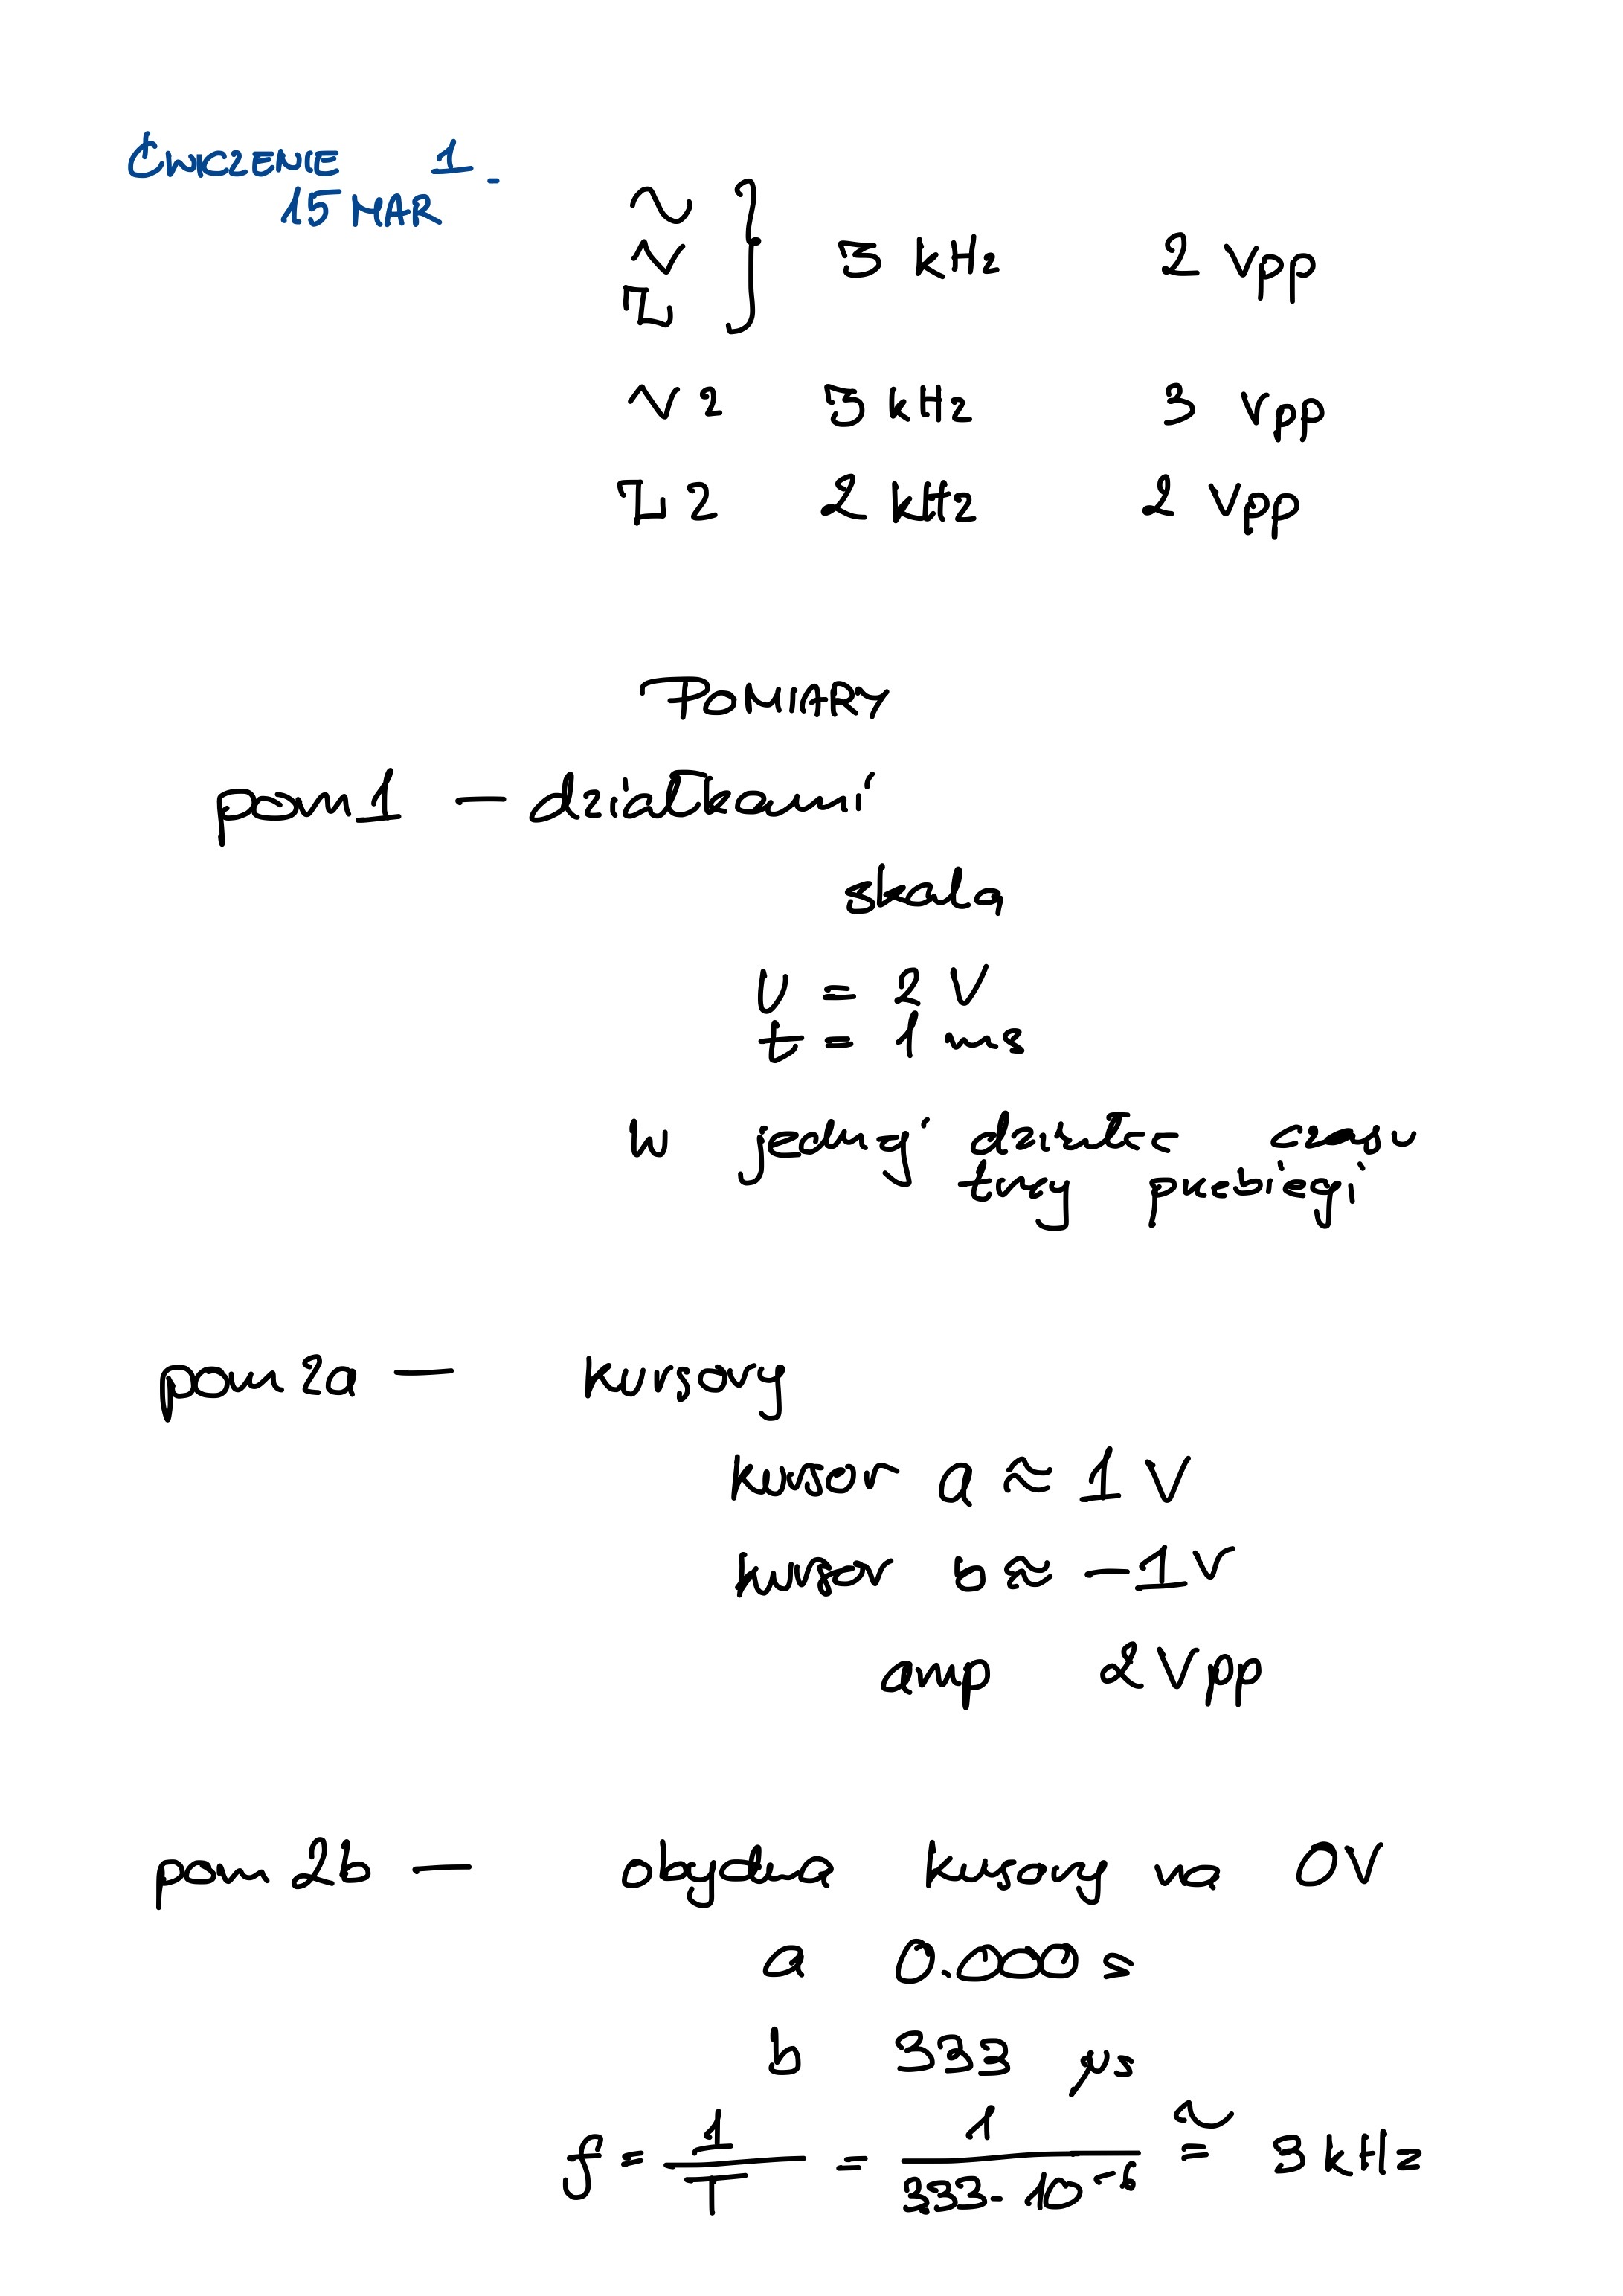
\includegraphics[scale=0.2]{B0}
\centering
\captionsetup{labelformat=empty}
\caption{}
\end{figure}

\begin{figure}[H]
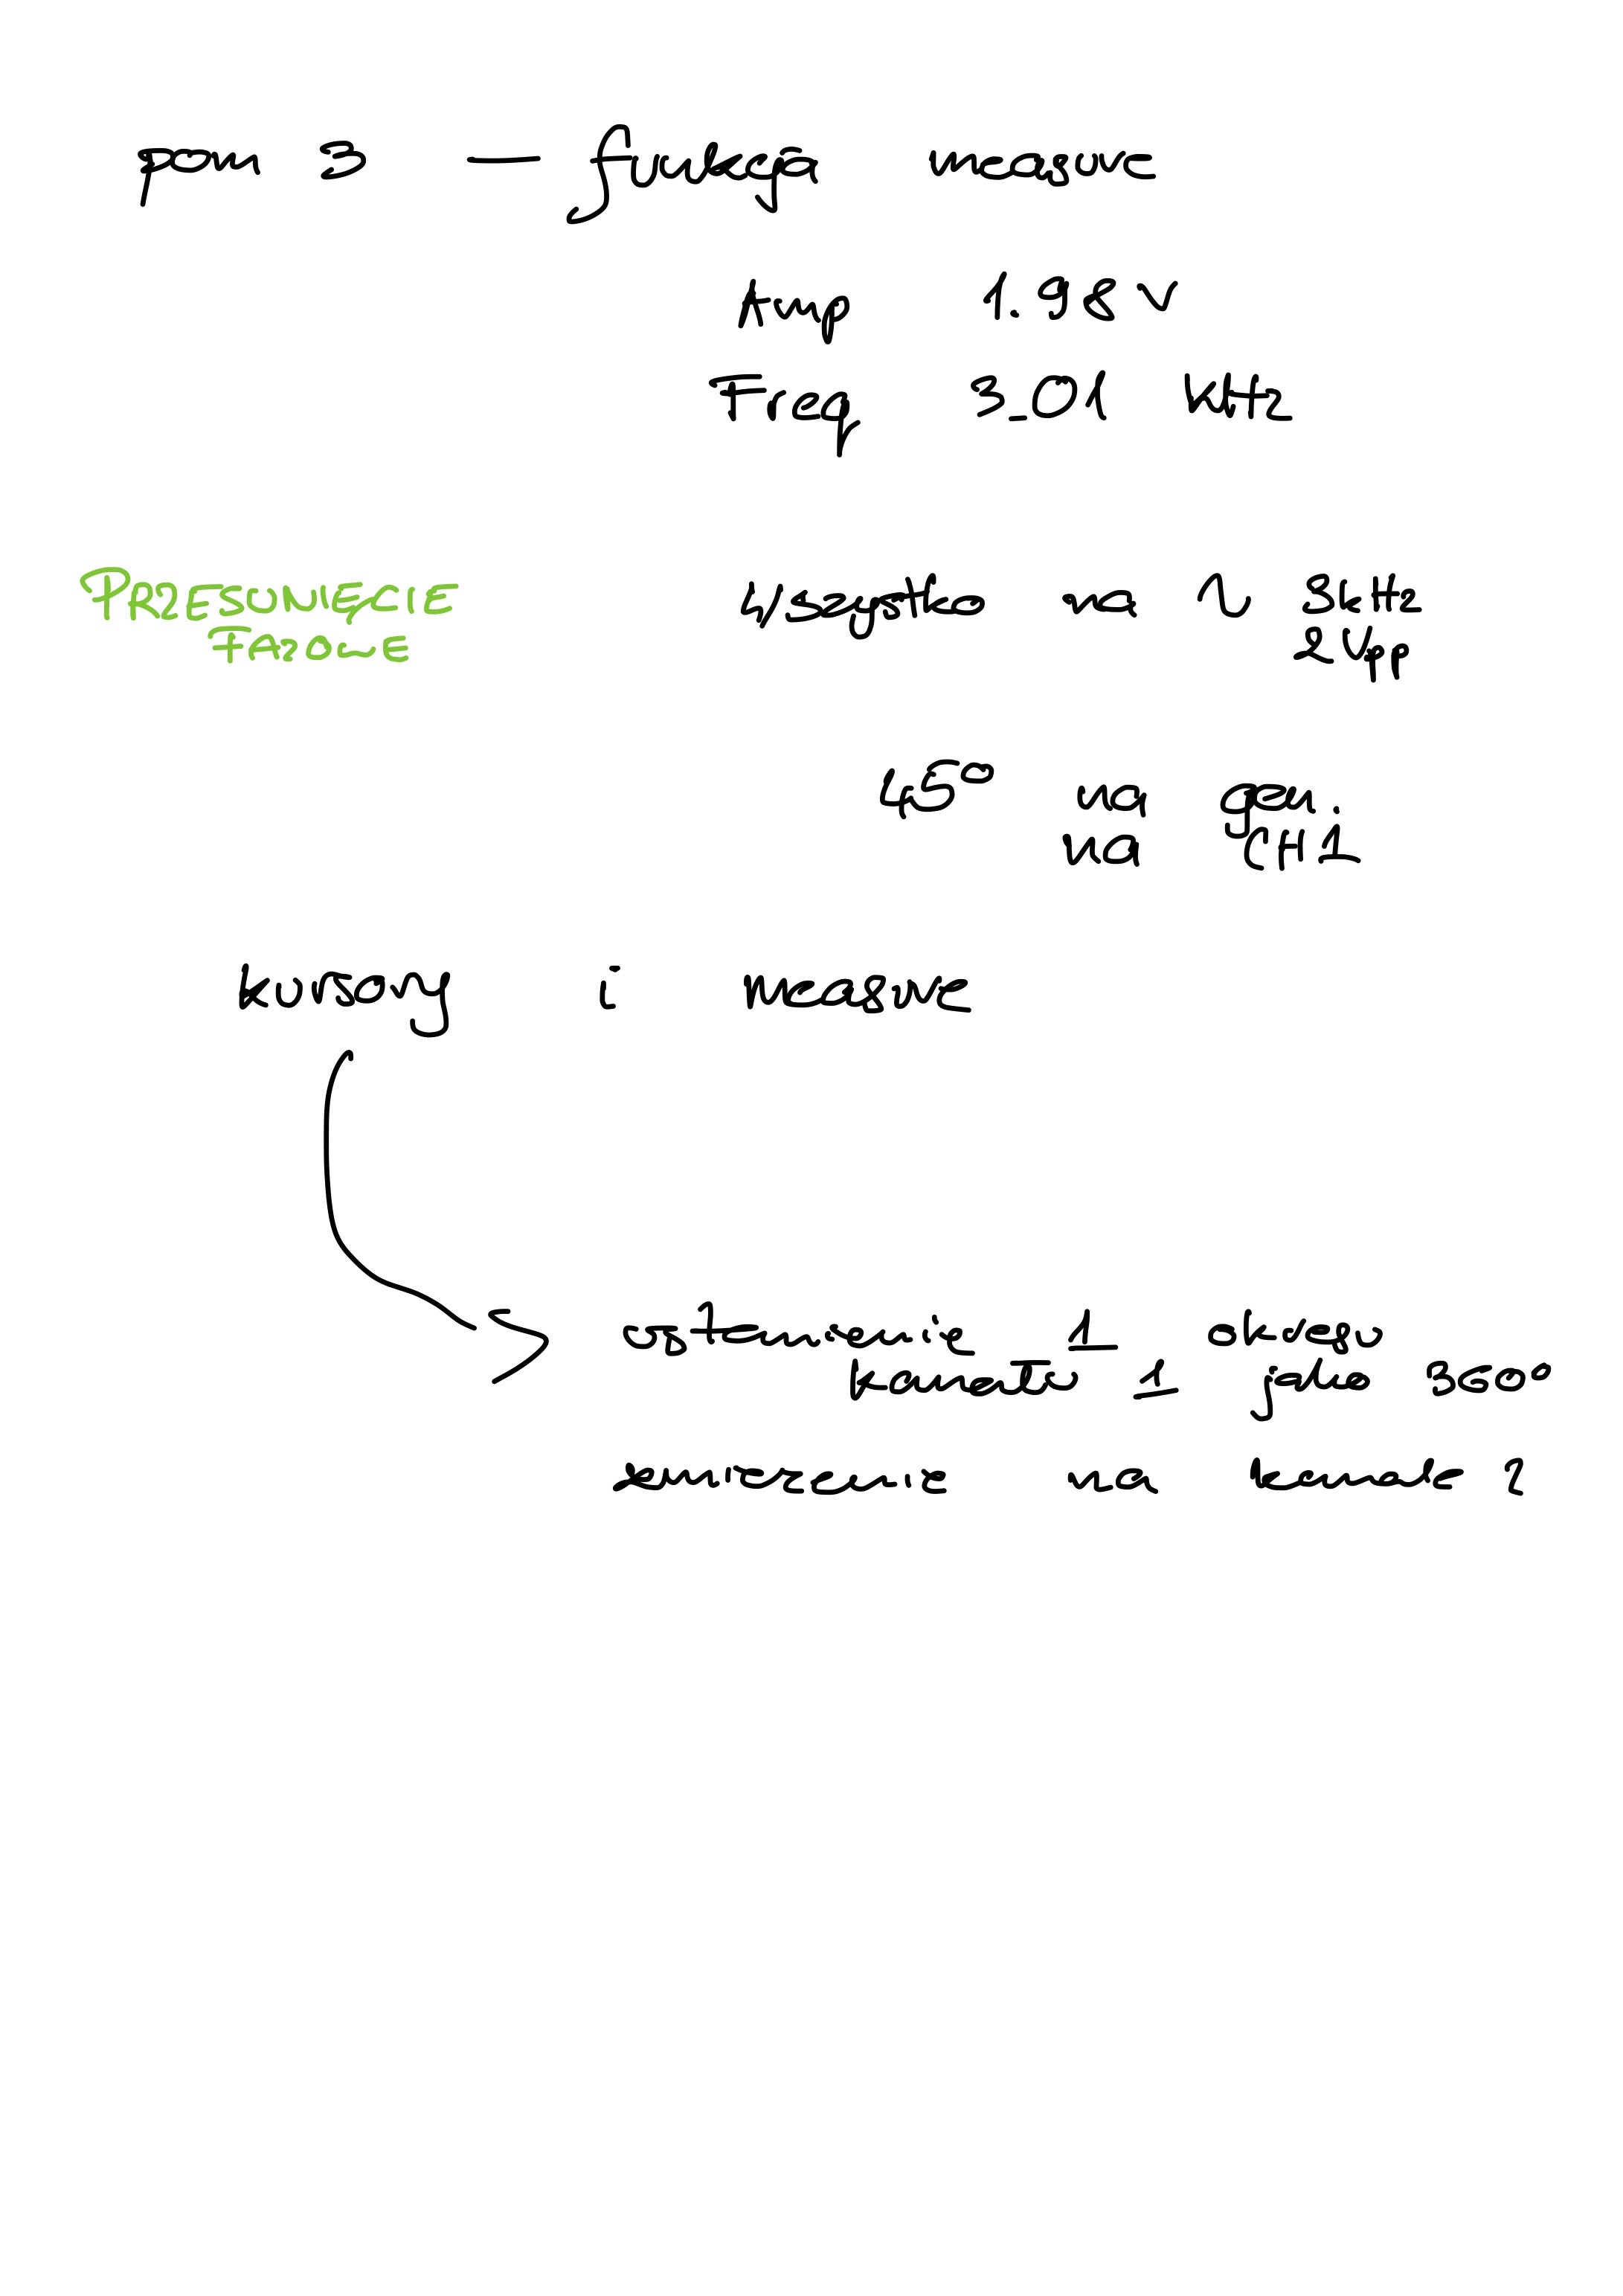
\includegraphics[scale=0.2]{B1}
\centering
\captionsetup{labelformat=empty}
\caption{}
\end{figure}

\begin{figure}[H]
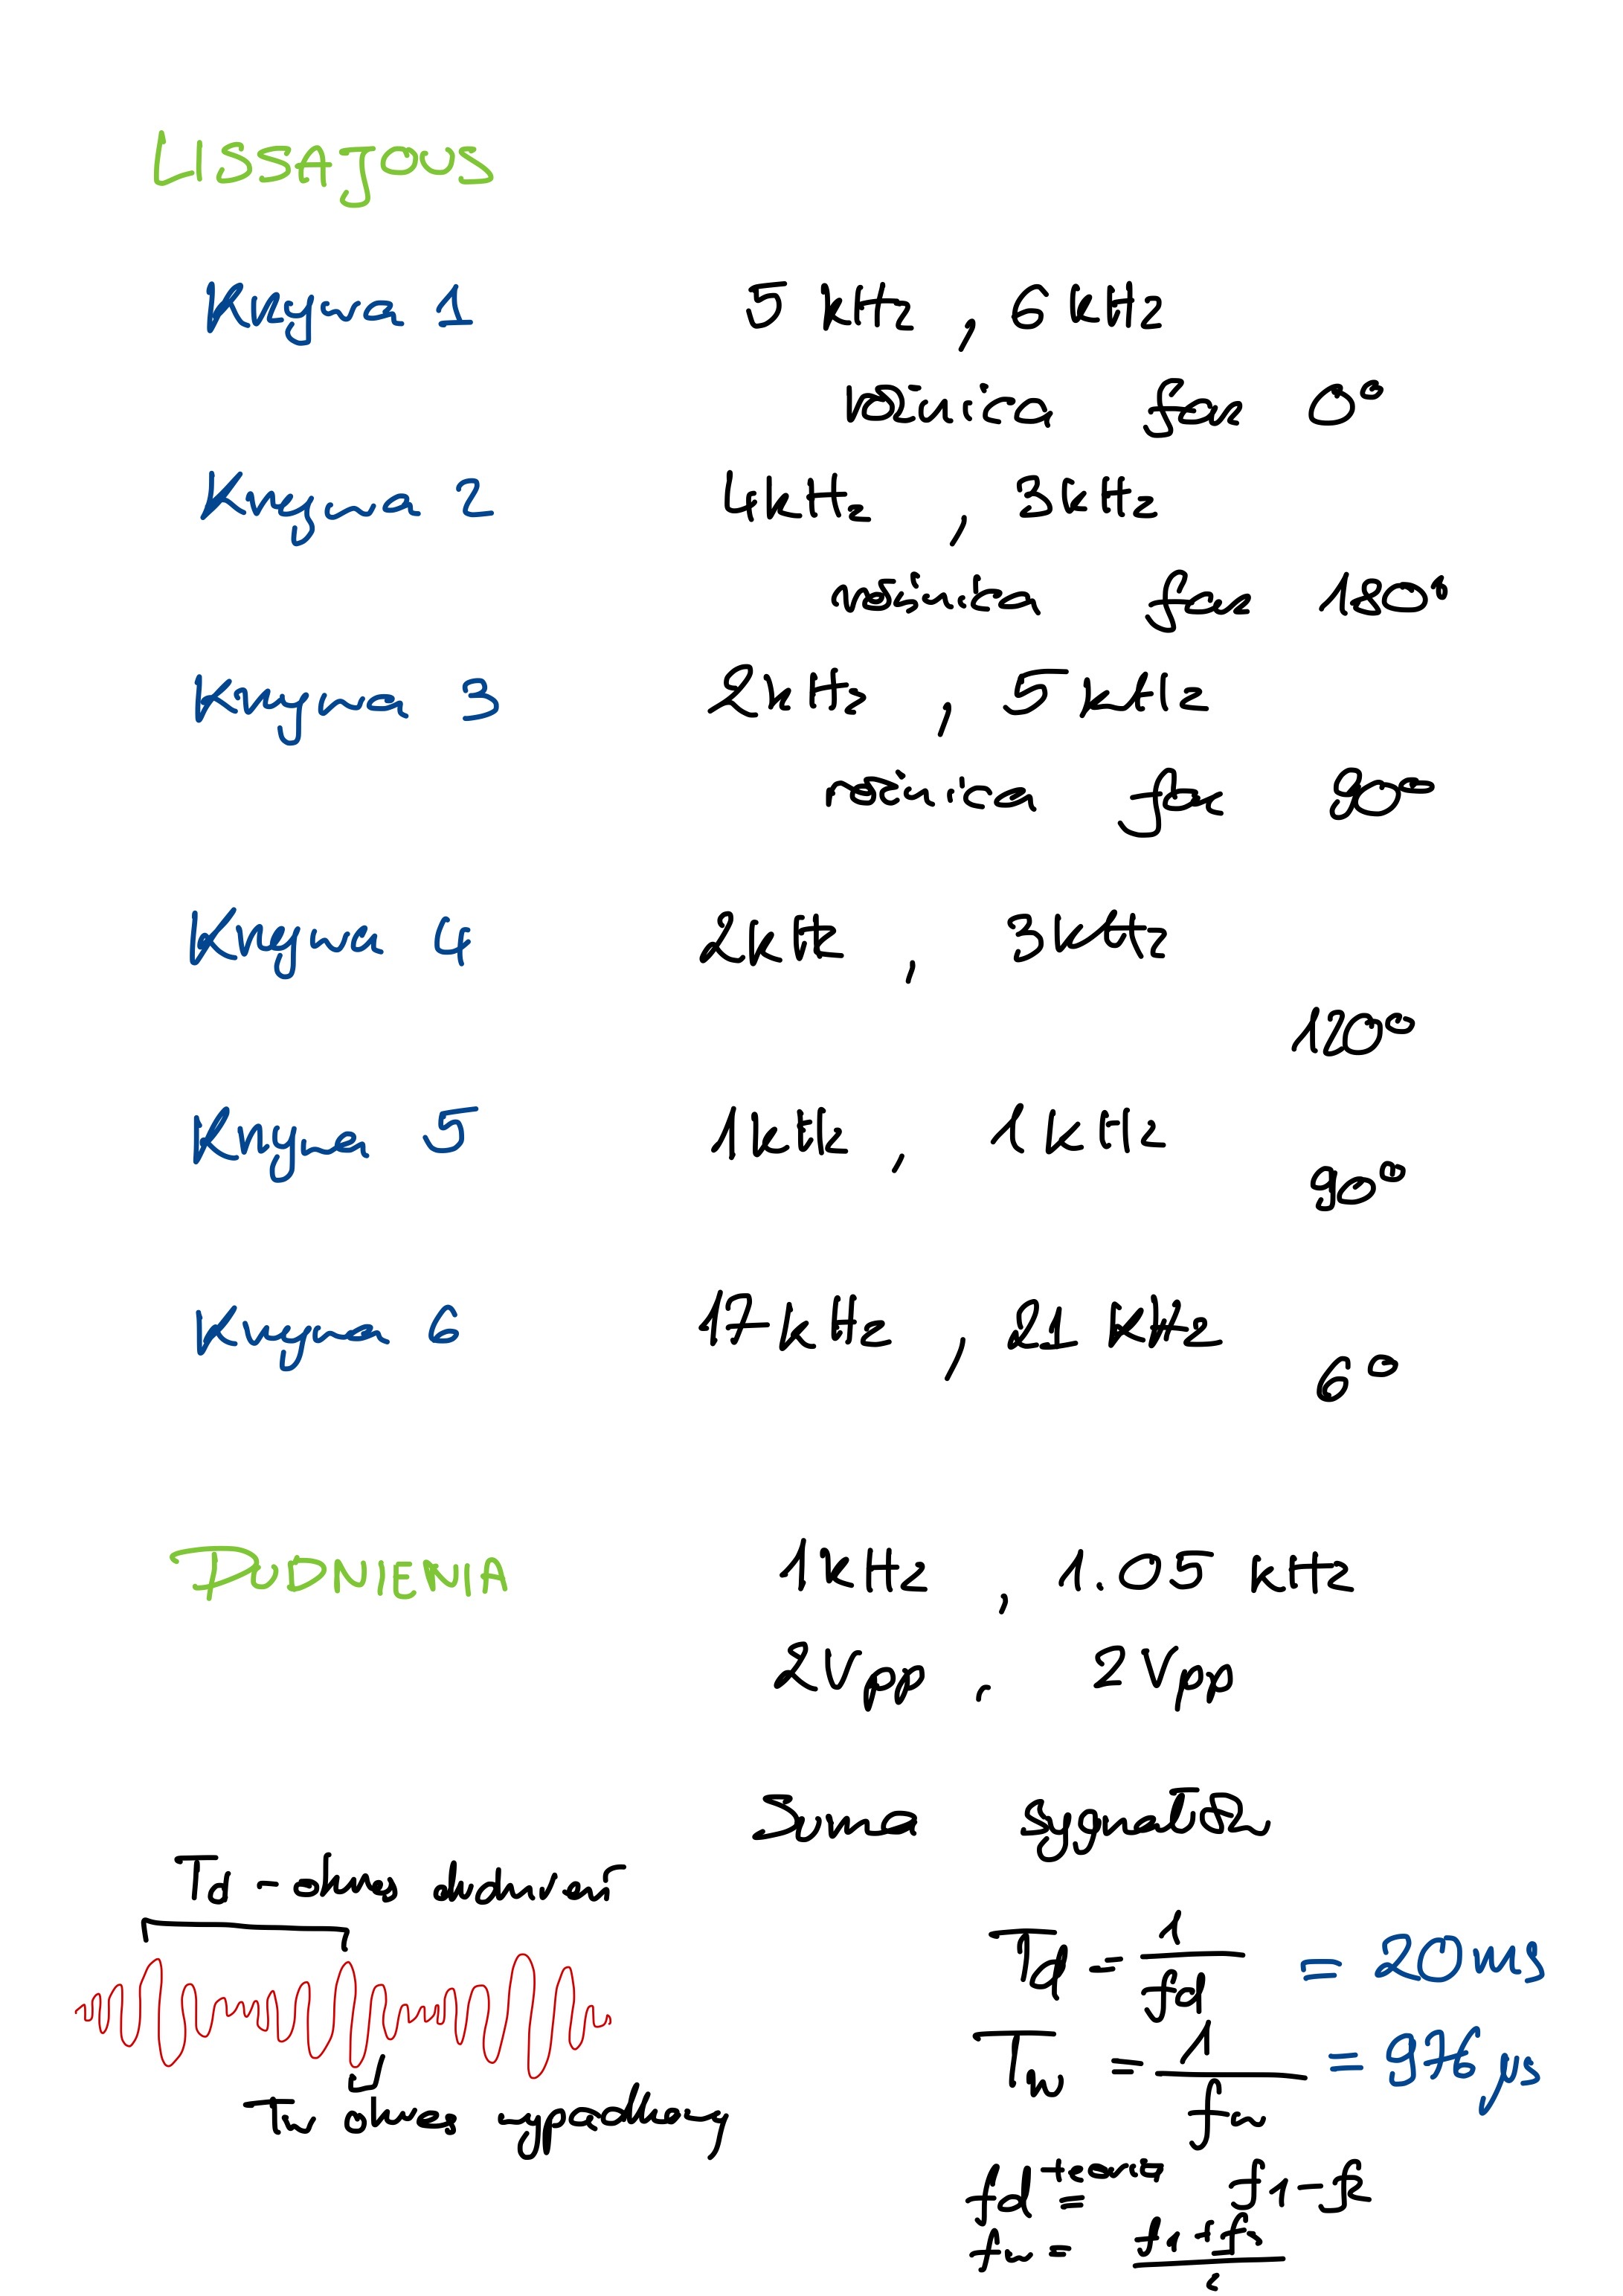
\includegraphics[scale=0.2]{B2}
\centering
\captionsetup{labelformat=empty}
\caption{}
\end{figure}

\end{document}